\subsubsection{ADI and AEI Visualization}
The ADI and AEI indices measure the diversity and evenness of sounds in a sound file, usually used to draw conclusions as to the diversity of animals at the site. For these indices, a single value is used to represent their values. The algorithms used in this service provide both a right and left channel ADI and AEI value where relevant, along with band values for each frequency range tested. Thus, a single numerical value representation for single file or dataset analysis is available, along with a graph showing these values at each band range. However for comparing ADI and AEI across data sets, it may be more beneficial to use these single values to create a line graph. See the comparison section for more details on this. In addition, it is useful to compare the ADI and AEI, so when the user measures \textit{both} indices on a file or data set, the service will compare them appropriately using a line graph.\\

\begin{center}
	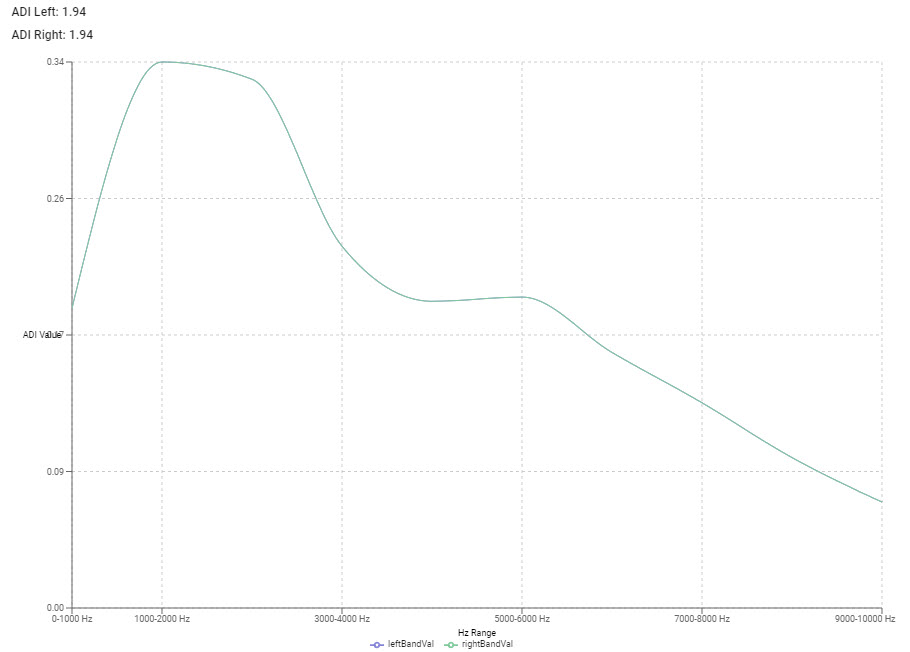
\includegraphics[width=\textwidth]{ADIgraph1} \\[12pt]
\end{center}
The first graph available for ADI and AEI is a line chart for displaying the ADI value at each frequency band range. The lines represent each channel, however in the image above the sound file used was single channeled.\\

\begin{center}
	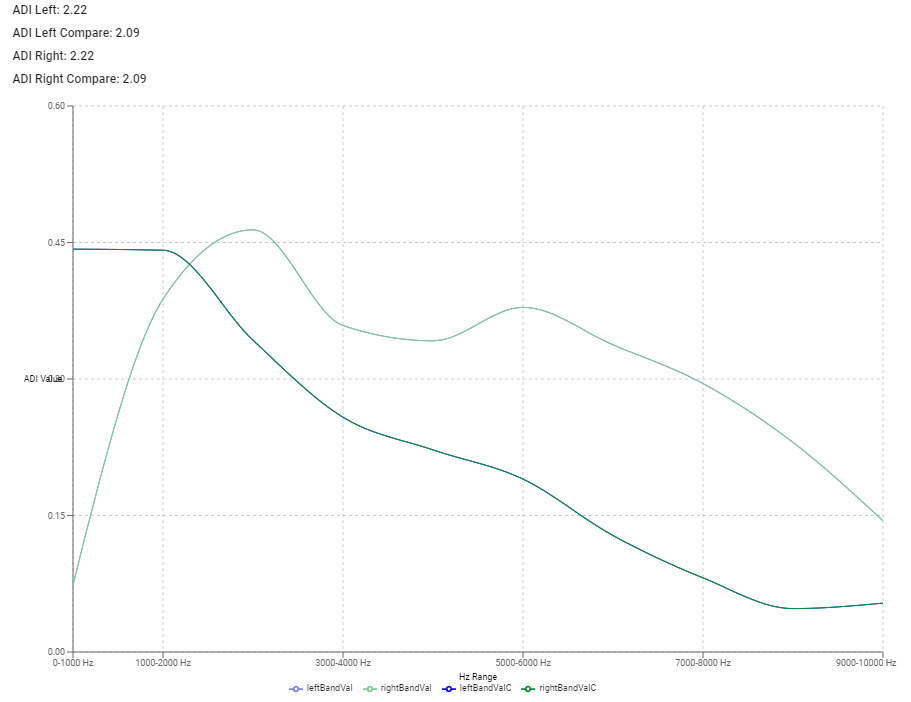
\includegraphics[width=\textwidth]{ADIgraph2} \\[12pt]
\end{center}
The second visualization available is similar to the first, however this one is for comparing individual files in the data set. Each line represents the respective file and its channel values.\\

\begin{center}
	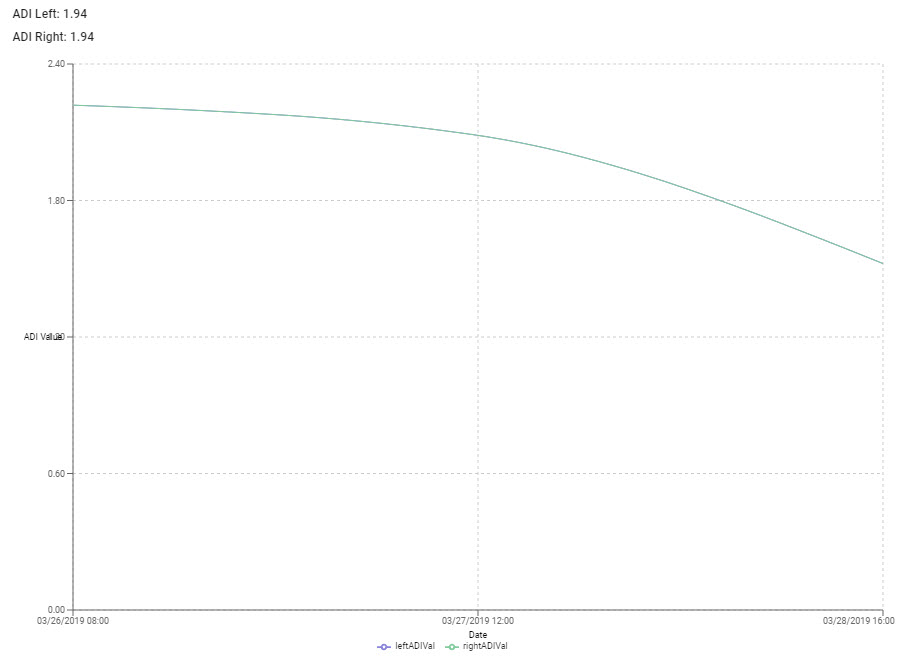
\includegraphics[width=\textwidth]{ADIgraph3} \\[12pt]
\end{center}
Finally, the last graph available for ADI and AEI is a line graph for displaying the index value over date and time and by file. Both graphs are line graphs and display very similarly, so only one is shown above.
